\documentclass[10pt]{beamer}
\usepackage[utf8]{inputenc}
\usepackage[czech]{babel}
\usepackage[abs]{overpic}

\usetheme[progressbar=frametitle]{metropolis}
\usepackage{appendixnumberbeamer}

\usepackage{booktabs}
\usepackage[scale=2]{ccicons}

\usepackage{pgfplots}
\usepgfplotslibrary{dateplot}

\usepackage{xspace}
\newcommand{\themename}{\textbf{\textsc{metropolis}}\xspace}
\definecolor{mSybilaRed}{HTML}{870004}

\setbeamercolor{title separator}{
  fg=mSybilaRed
}

\setbeamercolor{progress bar}{%
  fg=mSybilaRed,
  bg=mSybilaRed!90!black!30
}

\setbeamercolor{progress bar in section page}{
  use=progress bar,
  parent=progress bar
}

\setbeamercolor{alerted text}{%
  fg=mSybilaRed
}
\usepackage{color}

\definecolor{mygreen}{RGB}{51, 169, 54}

\title{Formálny biochemický priestor pre špecifikáciu a analýzu biochemických procesov}
%Formal Biochemical Space for Specification and Analysis of Biochemical Processes} 
\subtitle{Obhajoba diplomovej práce}
\author[Matej Troják]{Matej Troják}
\date{Fakulta Informatiky, Brno, 5.2.2018}

\titlegraphic{\hfill
\includegraphics[height=0.6cm]{sybila-simple.png}}

\setbeamertemplate{footline}
{
  \leavevmode
  \hbox{
  \begin{beamercolorbox}[wd=.15\paperwidth,ht=2.25ex,dp=1ex,center]{title in head/foot}
    \usebeamerfont{author in head/foot}\insertshortauthor
  \end{beamercolorbox}

  \begin{beamercolorbox}[wd=.7\paperwidth,ht=2.25ex,dp=1ex,center]{author in head/foot}
    \usebeamerfont{author in head/foot}\insertshorttitle
  \end{beamercolorbox}

  \begin{beamercolorbox}[wd=.15\paperwidth,ht=2.25ex,dp=1ex,center]{title in head/foot}
    \insertframenumber{} / \inserttotalframenumber
  \end{beamercolorbox}
  }
}

\begin{document}

\frame{
\thispagestyle{empty}
\titlepage
}

% -------------------------------------------------------------

\frame{
\frametitle{Motivácia}

Časté problémy s (biologickými) modelmi:

\begin{itemize}
\item rekonštrukcia -- "spustiteľný" ~model
\item pochopenie -- aký systém model predstavuje?
\item interpretácia -- čo model vysvetľuje?
\end{itemize}

\begin{center}
\vspace*{-1.5cm}
\includegraphics[width=0.8\textwidth]{motivation}
\end{center}

}
% -------------------------------------------------------------

\frame{
\frametitle{Riešenie -- Comprehensive Modelling Platform}

Webový framework pre \textbf{integráciu} biologických znalostí s výpočetnými modelmi a experimentami.

\begin{center}
\begin{columns}
\begin{column}{0.45\textwidth}

\begin{itemize}
	\item \url{e-photosynthesis.org}
\end{itemize}

\vspace{0.5cm}

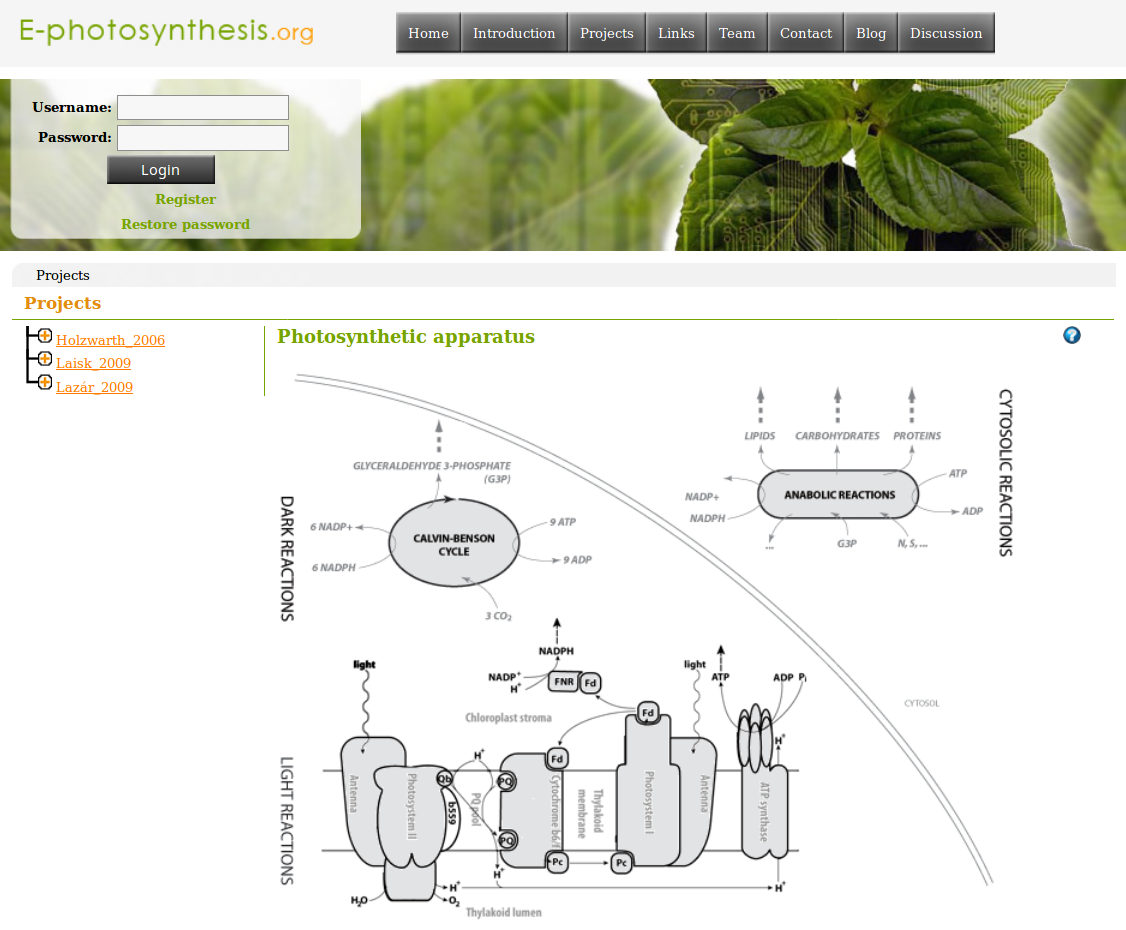
\includegraphics[width=1\textwidth]{ephoto}

\end{column}

\begin{column}{0.45\textwidth}

\begin{itemize}
	\item \url{e-cyanobacterium.org}
\end{itemize}

\vspace{0.5cm}

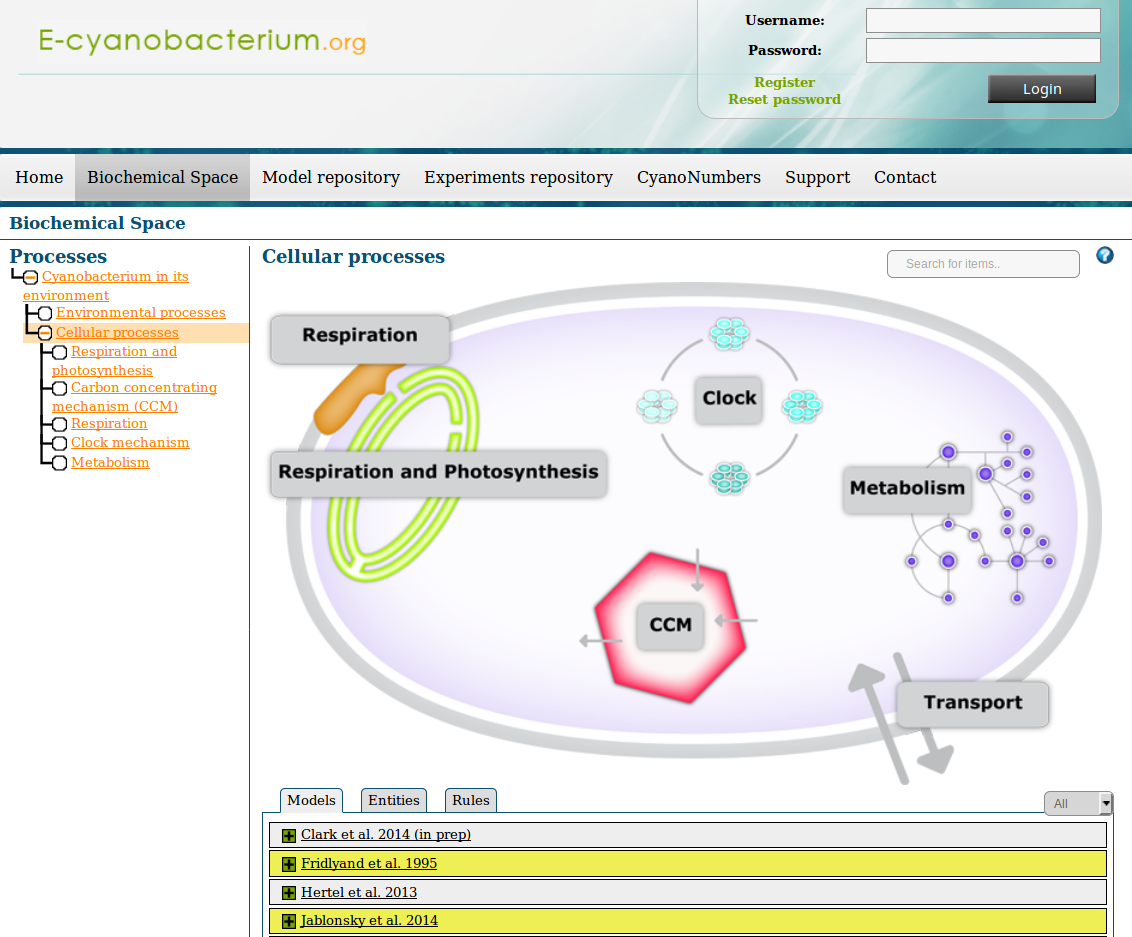
\includegraphics[width=1\textwidth]{ecyano}

\end{column}
\end{columns}
\end{center}
}

% -------------------------------------------------------------

\frame{
\frametitle{Biochemický priestor}

\textbf{Biochemický priestor} (Biochemical Space -- BCS) je doména biologických znalostí s formálnymi prvkami, ktorá poskytuje 

\begin{itemize}
\item \textbf{popis},
\item anotáciu,
\item zdieľanie
\end{itemize}

špecificky zameraných biologických modelov.

\vspace{1cm}

\textbf{Motto}: \emph{formalizácia biologického popisu a anotácia modelov.}

}

% -------------------------------------------------------------

\frame{
\frametitle{Ciele práce}
  
\begin{center}
\begin{itemize}
	\item formálna definícia jazyka Biochemického priestoru,
	\begin{itemize}
		\item kompaktný zápis chemických reakcií tzv. \emph{rule-based} prístupom,
		\item abstrakcia od detailov chemických väzieb,
		\item hierarchické usporiadanie individuálych látok,
		\item spustiteľná sémantika,
	\end{itemize}
	\item návrh analyzačných techník pre tento jazyk,
	\item prototypová implementácia na editovanie a analyzovanie modelov zapísaných v tomto jazyku.
\end{itemize}
\end{center}

}


% -------------------------------------------------------------

\frame{
\frametitle{Ako to funguje}
  
\begin{center}
 \hspace*{-0.7cm}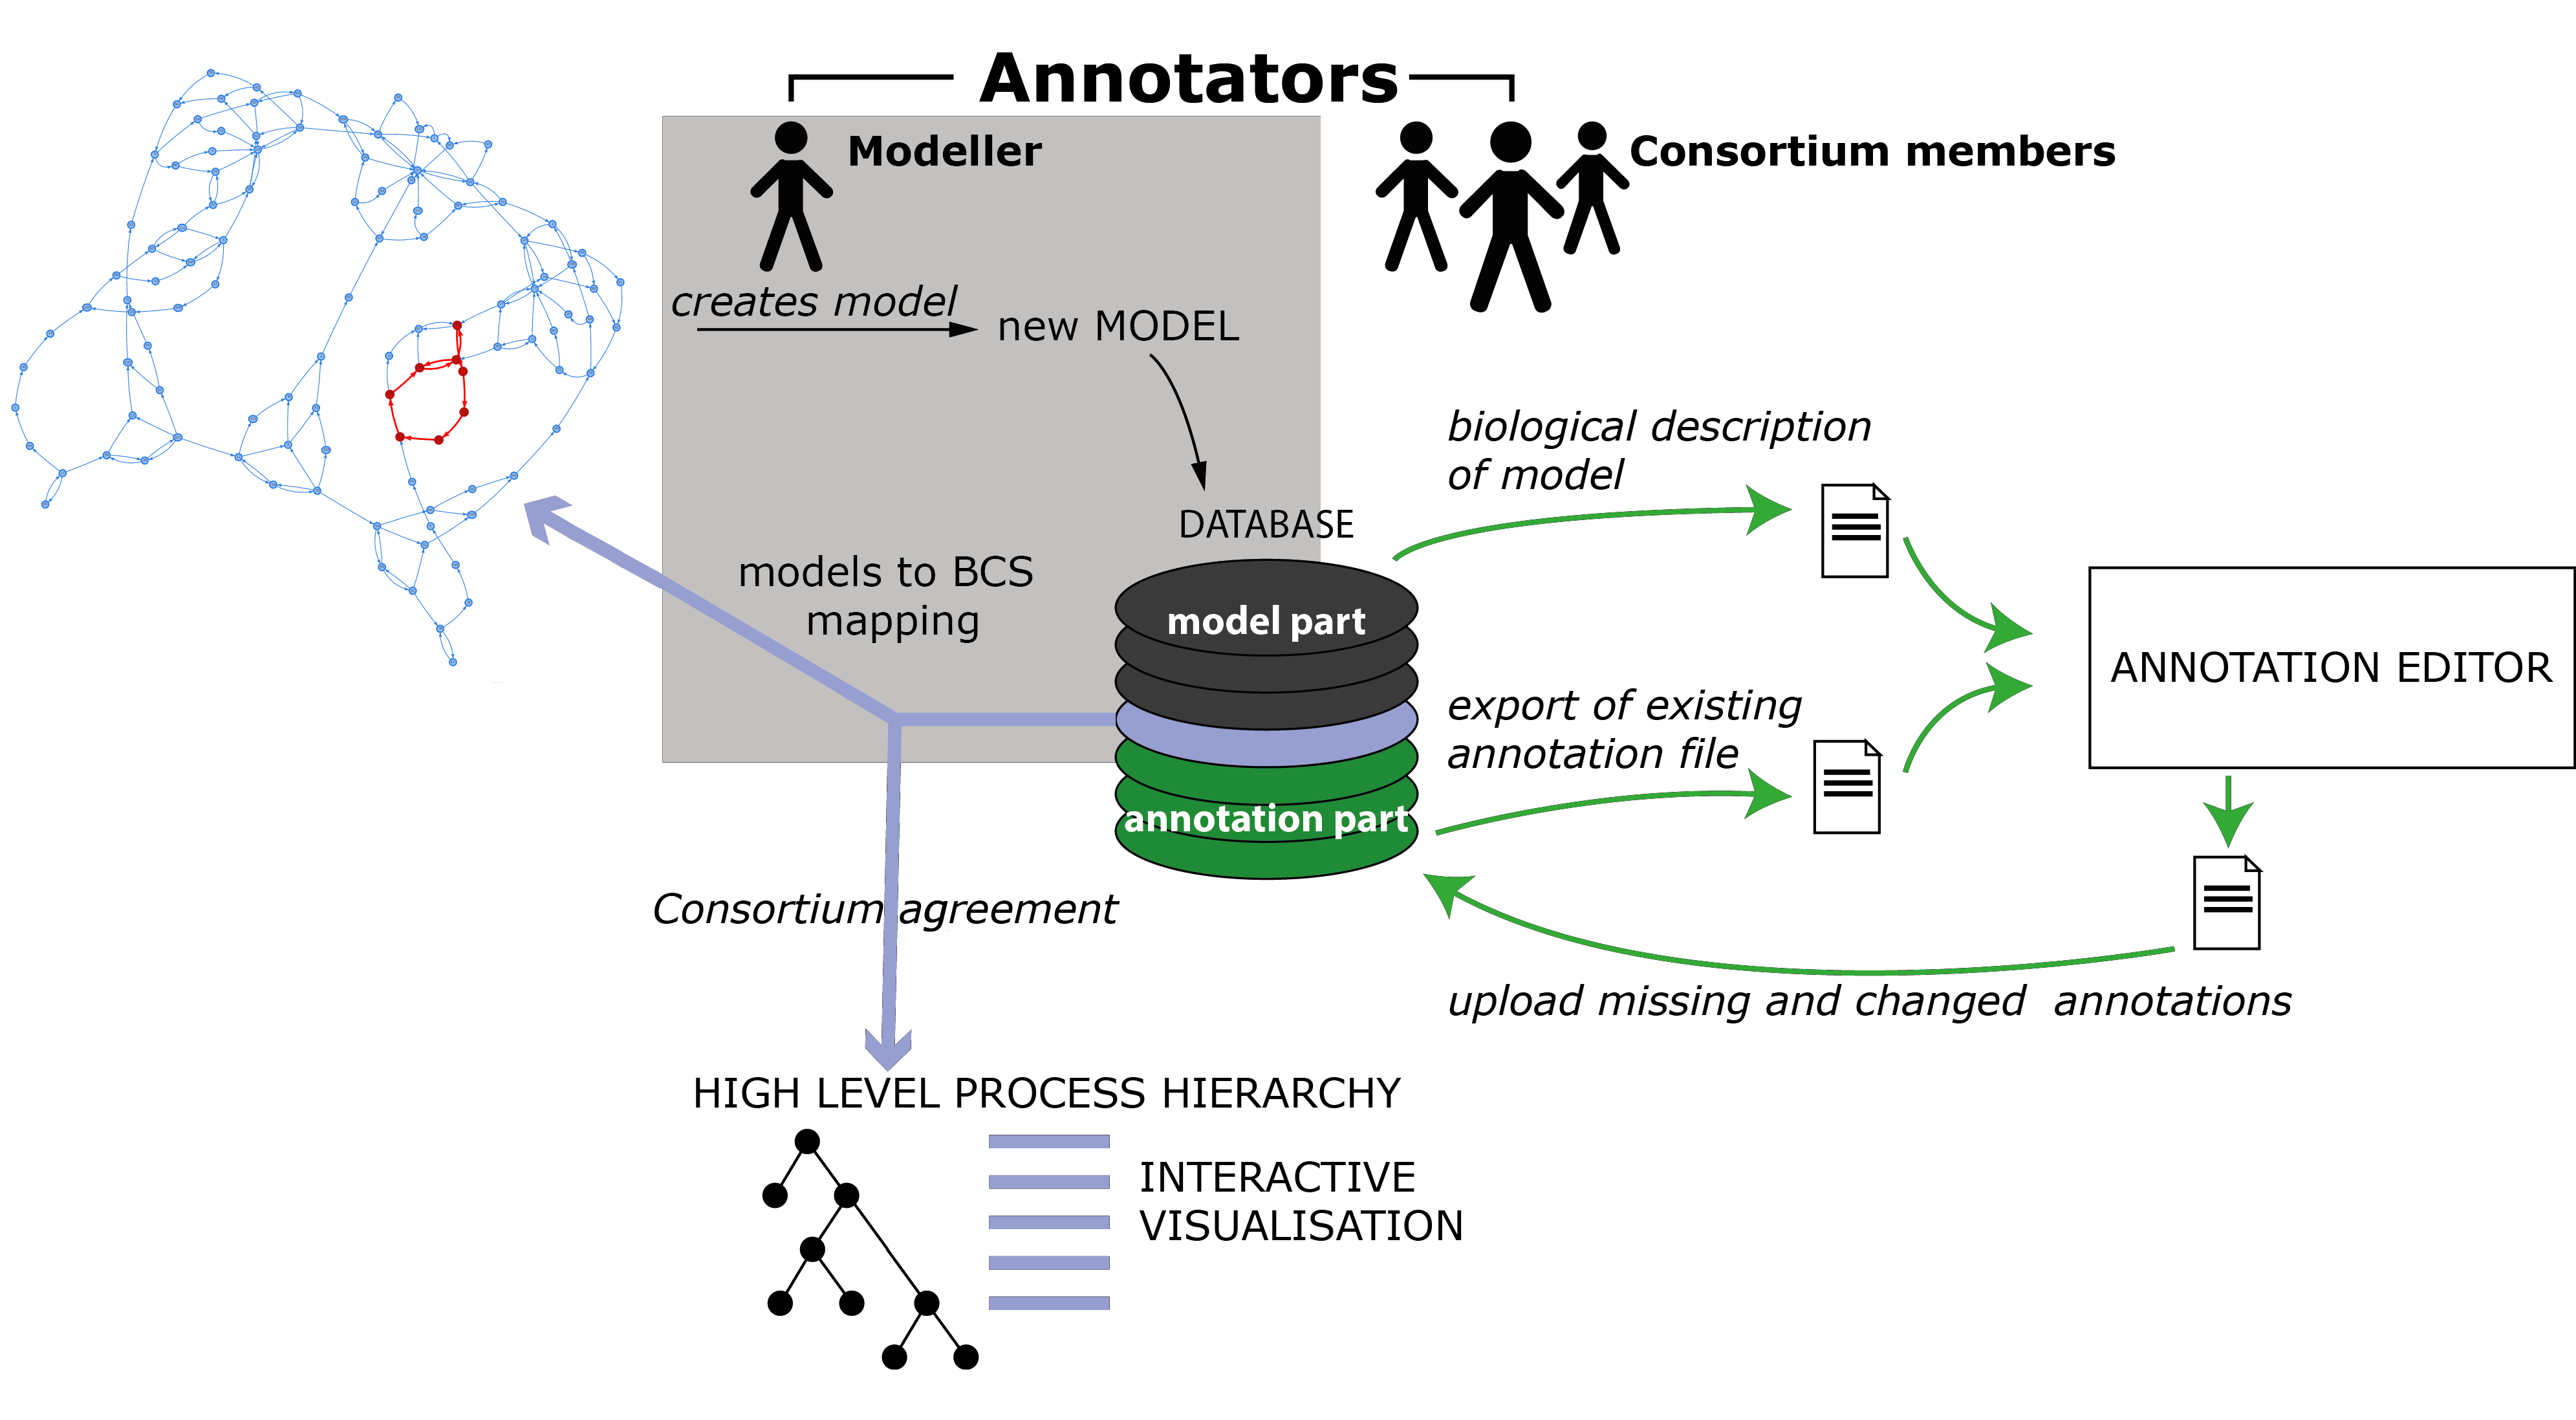
\includegraphics[width=1.1\textwidth]{annot}
\end{center}

}

% -------------------------------------------------------------

\frame{
\frametitle{Výhody}

\begin{itemize}
\item model získa svoj biologický význam

\begin{itemize}
\item anotácia pre individuálne componenty/reakcie vždy ľahko dostupná
\item implementovaný model dostupný online
\end{itemize}

\item vymedzením vzťahu model ku BCS získame popis modelu v BCSL

\begin{itemize}
\item možnosť ďalšej analýzy
\item jednotná forma modelov -- porovnávanie
\end{itemize}

\end{itemize}

\begin{center}

\includegraphics[width=0.8\textwidth]{transformation}
\end{center}

}

% -------------------------------------------------------------

\frame{
\frametitle{Databáza}

\begin{center}
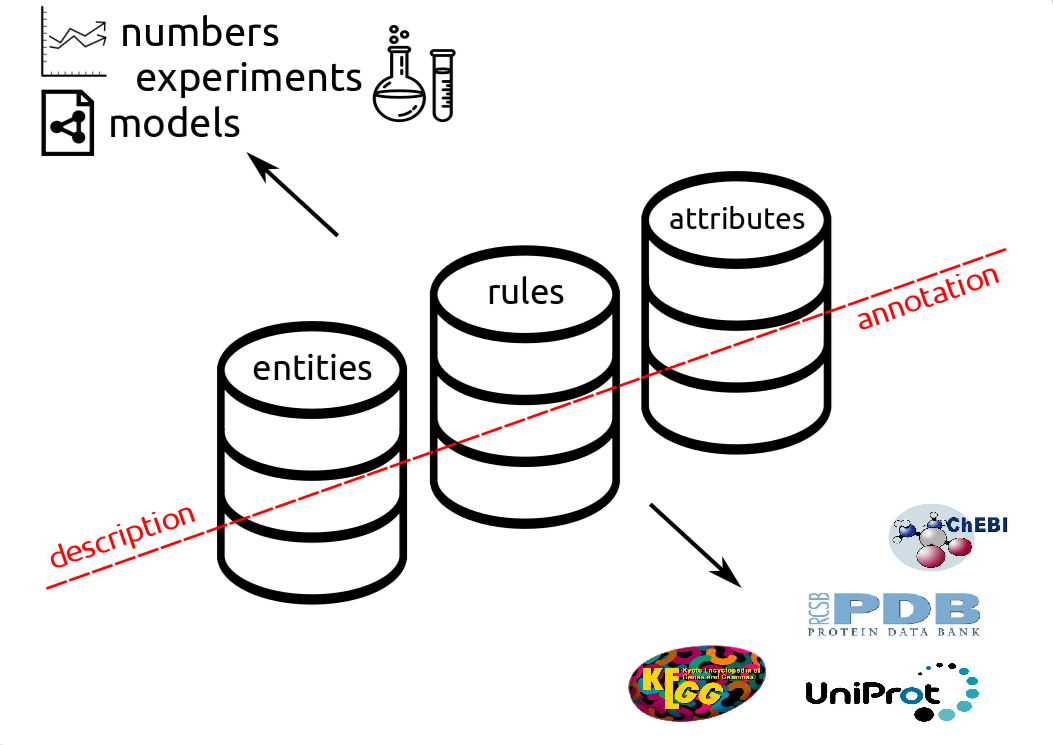
\includegraphics[width=1\textwidth]{bcs_database.png}
\end{center}

}


% -------------------------------------------------------------

\frame{
\frametitle{BCS formát}
  
\begin{center}
 \hspace*{-0.7cm}\includegraphics[width=1.1\textwidth]{equation}
\end{center}

}

% -------------------------------------------------------------

\frame{
\frametitle{Rule-based vs. reaction-based}
  
\begin{center}
 \hspace*{-0.7cm}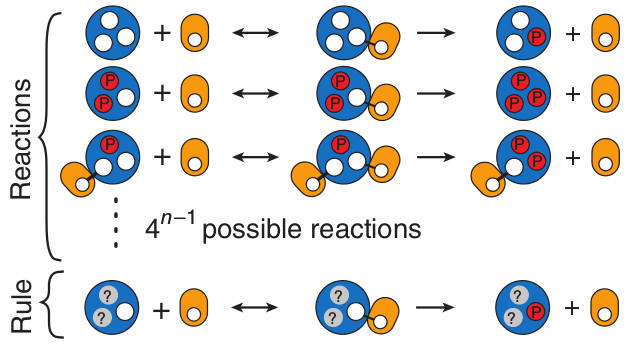
\includegraphics[width=0.9\textwidth]{reaction_vs_rule}
\end{center}

}

% -------------------------------------------------------------

\frame{
\frametitle{Entity}
  
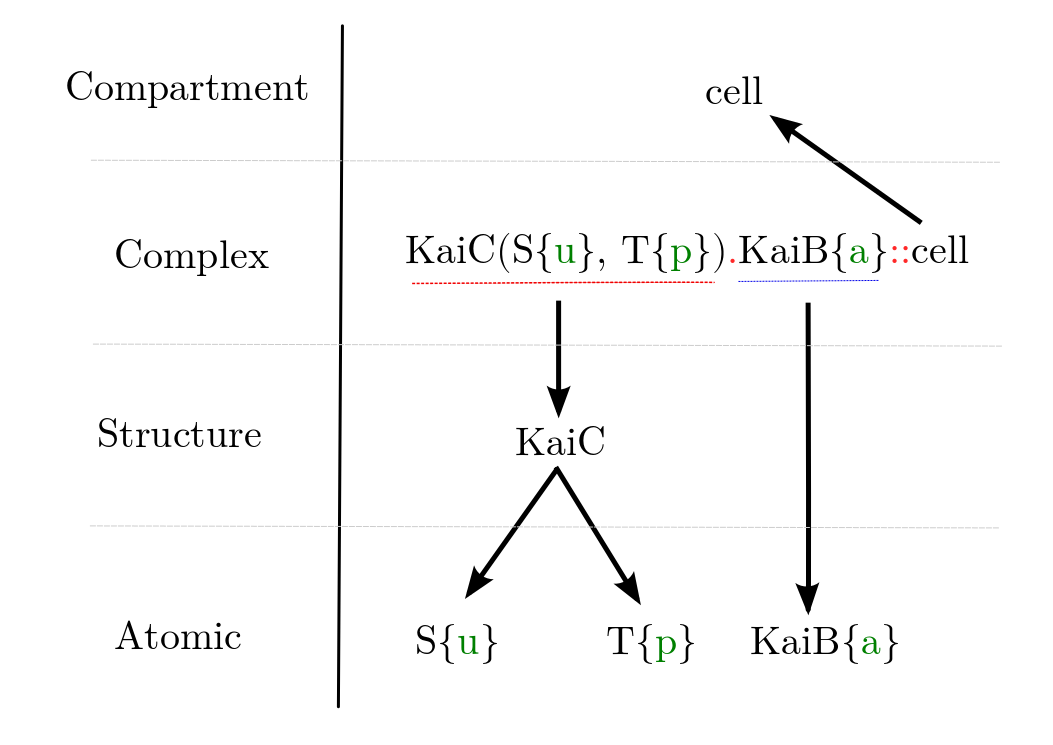
\includegraphics[width=1\textwidth]{hierarchy}

}

% -------------------------------------------------------------

\frame{
\frametitle{Abstrakcia komplexu}
  
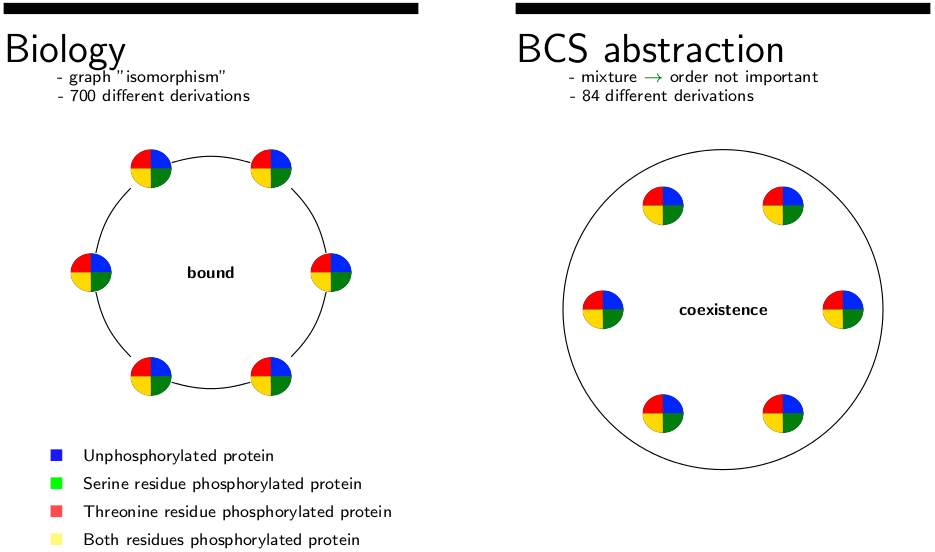
\includegraphics[width=1\textwidth]{abstraction}

}

% -------------------------------------------------------------

\frame{
\frametitle{Pravidlá}

\begin{center}
\begin{columns}
\begin{column}{0.9\textwidth}

E + S $\leftrightarrow$ ES

ES $\rightarrow$ E + P

\end{column}

\begin{column}{0.1\textwidth}
 

\includegraphics[width=.5\textwidth]{cross-mark}

\end{column}
\end{columns}

\vspace{.5cm}
\noindent\makebox[\linewidth]{\rule{1.1\textwidth}{0.4pt}}
\vspace{.2cm}

\begin{columns}
\begin{column}{0.9\textwidth}

E + S\{\textcolor{mygreen}{i}\} $\Rightarrow$ E\textcolor{red}{.}S\{\textcolor{mygreen}{u}\}

E\textcolor{red}{.}S\{\textcolor{mygreen}{u}\} $\Rightarrow$ E\textcolor{red}{.}S\{\textcolor{mygreen}{a}\}

E\textcolor{red}{.}S $\Rightarrow$ E + S 

\end{column}

\begin{column}{0.1\textwidth}
 

\includegraphics[width=.5\textwidth]{check-mark}

\end{column}
\end{columns}

\vspace{.5cm}
\noindent\makebox[\linewidth]{\rule{1.1\textwidth}{0.4pt}}
\vspace{.2cm}

\begin{columns}
\begin{column}{0.9\textwidth}

{\small R\textcolor{red}{(}$\mathtt{active}$\{\textcolor{mygreen}{off}\}, $\mathtt{enzyme}$\{\textcolor{mygreen}{avail}\}\textcolor{red}{)} $\Rightarrow$ R\textcolor{red}{(}$\mathtt{active}$\{\textcolor{mygreen}{on}\}, $\mathtt{enzyme}$\{\textcolor{mygreen}{avail}\}\textcolor{red}{)} }\\

{\small R\textcolor{red}{(}$\mathtt{enzyme}$\{\textcolor{mygreen}{avail}\}\textcolor{red}{)}
$\Leftrightarrow$ R\textcolor{red}{(}$\mathtt{enzyme}$\{\textcolor{mygreen}{unavail}\}\textcolor{red}{)} }\\

\end{column}

\begin{column}{0.1\textwidth}
 

\includegraphics[width=.5\textwidth]{check-mark}

\end{column}
\end{columns}
\end{center}

}

% -------------------------------------------------------------

\frame{
\frametitle{BCS doména umožňuje syntaktické rozšírenia}

\begin{columns}
\begin{column}{0.5\textwidth}

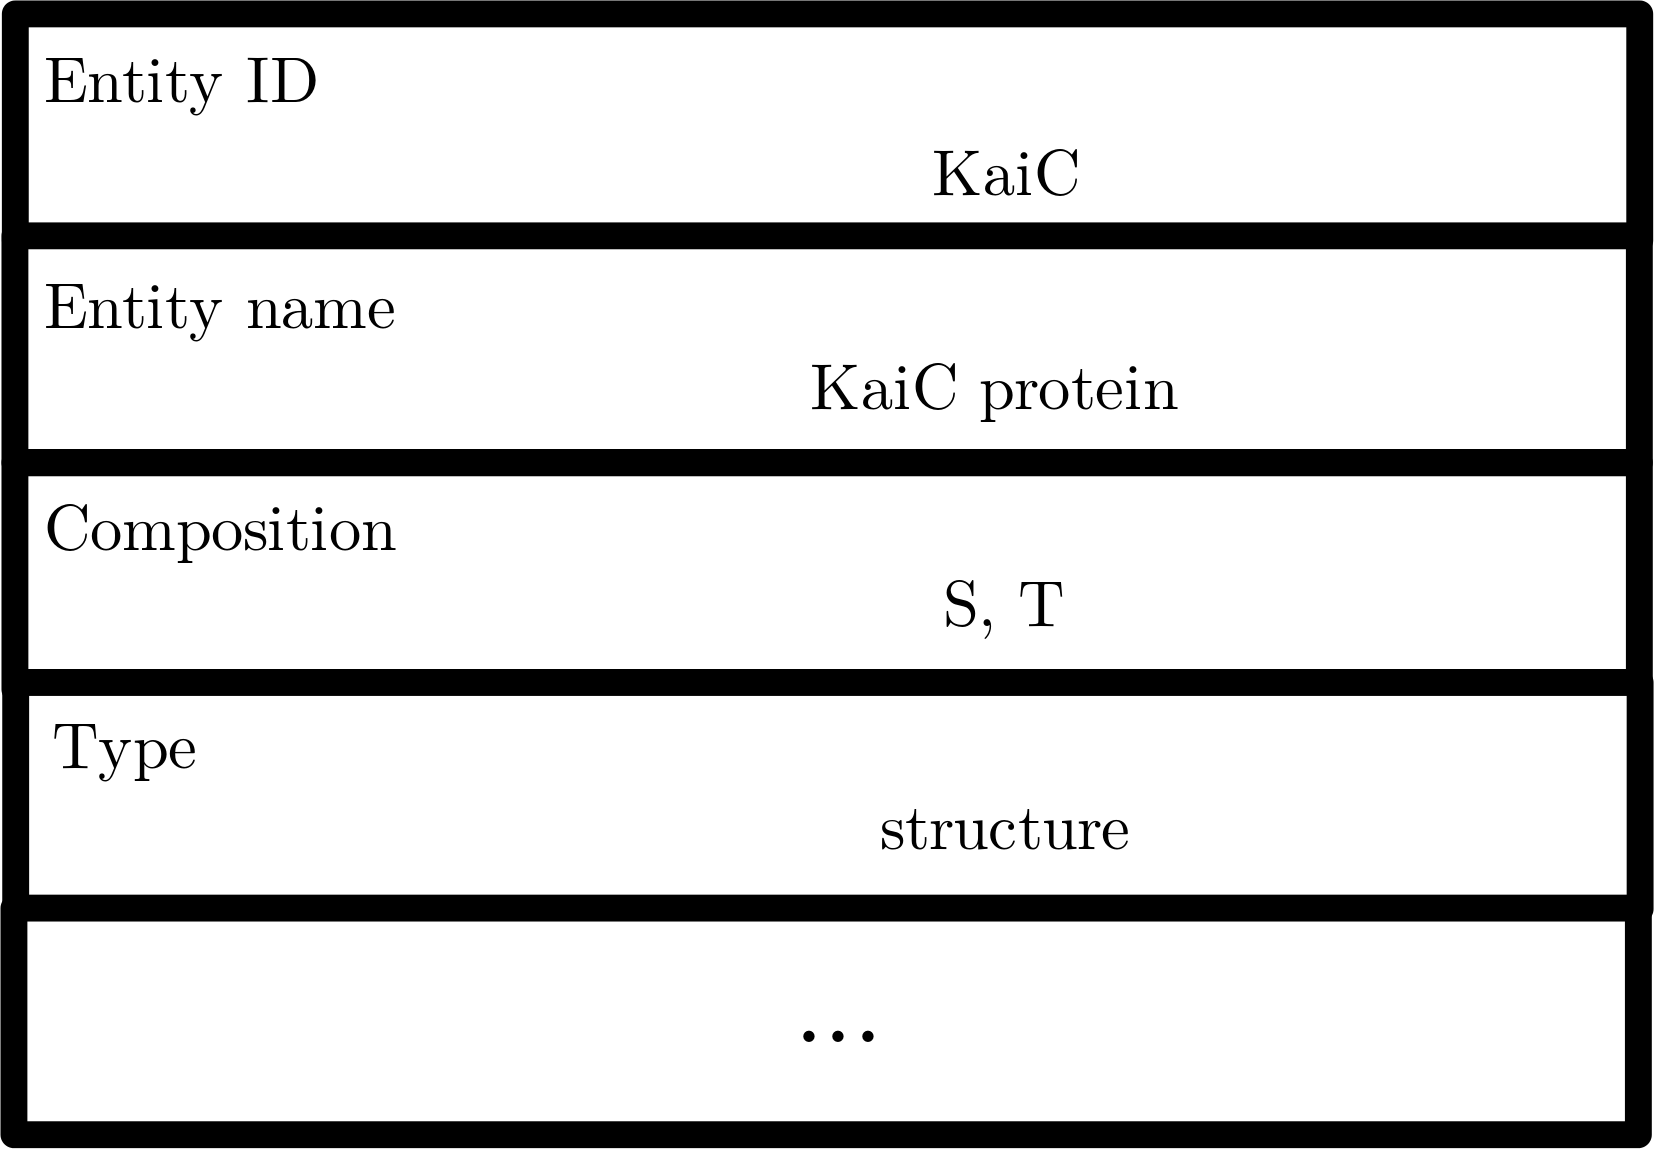
\includegraphics[width=1\textwidth]{entity_kaiC}

\end{column}

\begin{column}{0.5\textwidth}
  
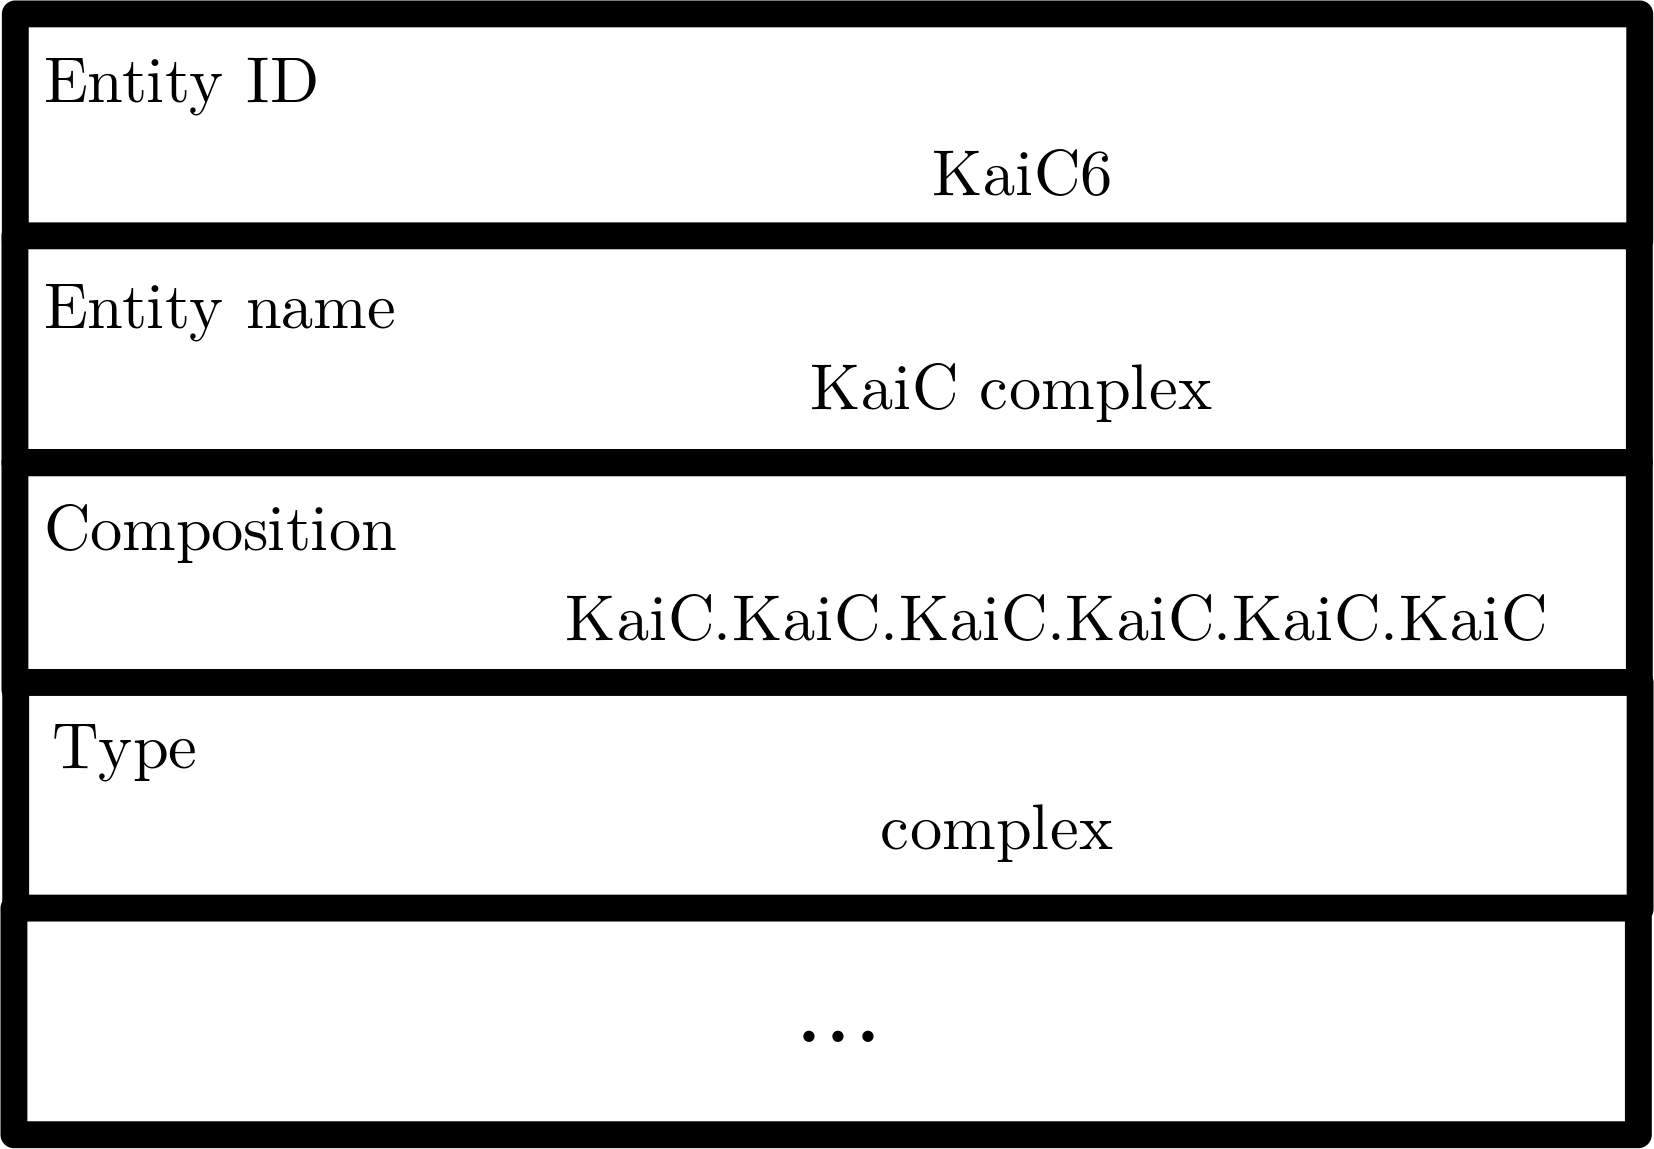
\includegraphics[width=1\textwidth]{entity_kaiC6}

\end{column}
\end{columns}

\vspace{0.5cm}\noindent\makebox[\linewidth]{\rule{1.1\textwidth}{0.4pt}}

\begin{center}

S\{\textcolor{mygreen}{u}\}::KaiC::KaiC6::cyt $\Rightarrow$ S\{\textcolor{mygreen}{p}\}::KaiC::KaiC6::cyt

\textcolor{red}{$\downarrow$}

KaiC(S\{\textcolor{mygreen}{u}\}).KaiC.~\ldots~.KaiC::cyt $\Rightarrow$ KaiC(S\{\textcolor{mygreen}{p}\}).KaiC.~\ldots~.KaiC::cyt

\end{center}

}

% -------------------------------------------------------------

\begin{frame}[standout]
\thispagestyle{empty}
  {\huge \href{https://www.youtube.com/watch?v=YwKIwoqVeJs}{Demo} \\}
\end{frame}

% -------------------------------------------------------------

\begin{frame}[standout]
\thispagestyle{empty}
  {\huge Ďakujem za pozornosť. \\}

  \vspace{2cm}

  {\huge Otázky? \\}
\end{frame}

% -------------------------------------------------------------

\appendix

% -------------------------------------------------------------

\frame{
\frametitle{Otázky oponenta}

\begin{itemize}

\item Vo druhej kapitole sa spomína, že jazyk Kappa nedokáže vyjadriť obecný vzťah koexistenie bez udania štruktúry, je preto nutné zvoliť nejakú kruhovú/lineárnu štruktúru. Nedala by sa ale takáto vlastnosť vyjadriť úplným grafom?

\end{itemize}

\alt<1>{
\begin{center}
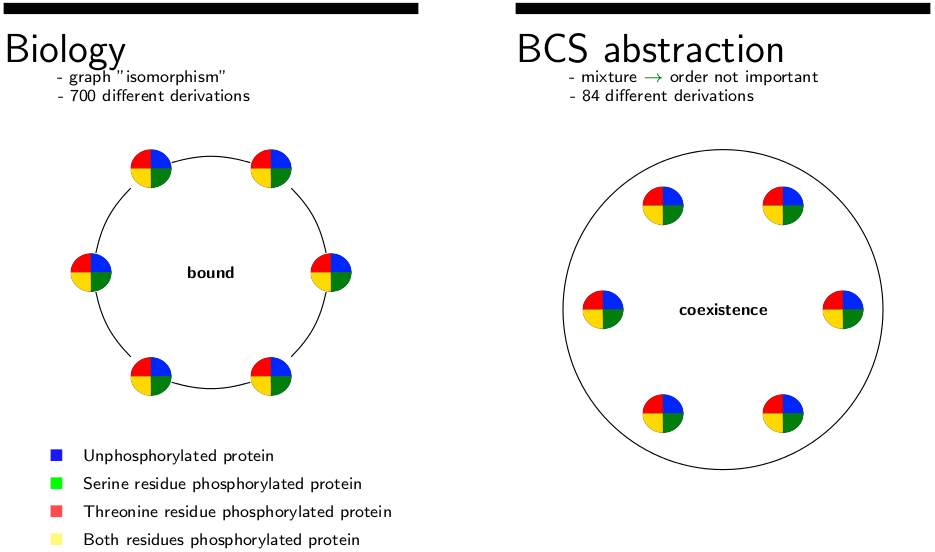
\includegraphics[width=0.8\textwidth]{abstraction}
\end{center}
}

\alt<2>{
\begin{center}
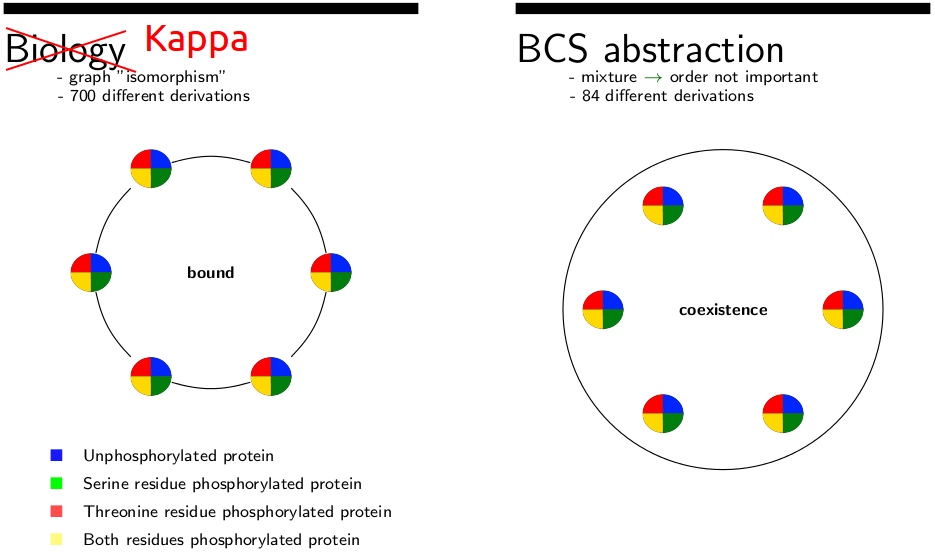
\includegraphics[width=0.8\textwidth]{abstraction_kappa}
\end{center}
}

\alt<3>{

\begin{columns}[T] % align columns
\begin{column}{.48\textwidth}

\begin{center}
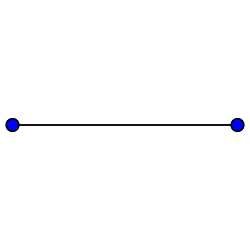
\includegraphics[width=0.4\textwidth]{Complete_graph_K2}

Node(bs!1), Node(bs!1)
\end{center}

\end{column}%
\hfill%
\begin{column}{.48\textwidth}

\begin{center}
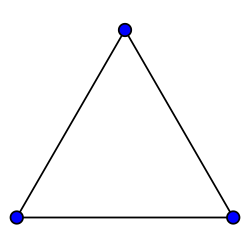
\includegraphics[width=0.4\textwidth]{Complete_graph_K3}

Node(bs1!1, bs2!2), 

Node(bs1!1, bs2!3), 

Node(bs1!3, bs2!2)
\end{center}

\end{column}%
\end{columns}

}

\alt<4>{

\begin{columns}[T] % align columns
\begin{column}{.29\textwidth}

\vspace{2cm}
{\hspace*{2cm}\huge \ldots \\}

\end{column}%
\hfill%
\begin{column}{.69\textwidth}

\begin{center}
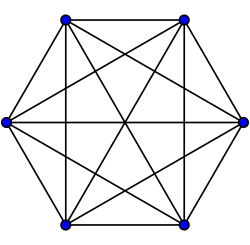
\includegraphics[width=0.3\textwidth]{Complete_graph_K6}

Node(bs1!1, bs2!2, bs3!3, bs4!4, bs5!5), 

Node(bs1!5, bs2!6, bs3!7, bs4!8, bs5!9), 

Node(bs1!9, bs2!4, bs3!10, bs4!11, bs5!12),

Node(bs1!12, bs2!8, bs3!3, bs4!13, bs5!14),

Node(bs1!14, bs2!11, bs3!7, bs4!2, bs5!15),

Node(bs1!15, bs2!13, bs3!10, bs4!6, bs5!1)
\end{center}

\end{column}%
\end{columns}

}

}

% -------------------------------------------------------------

\frame{
\frametitle{Otázky oponenta}

\begin{itemize}

\item Je nejaký dôvod prečo komplexný agent vo svojej definícií nedefinuje ako multiset, ale ako sekvenciu, ak (pokiaľ dobre vidím) sa všade aj tak táto sekvencia uvažuje len vzhľadom k všetkým jej permutáciám?

\end{itemize}

\begin{center}

\alt<1>{
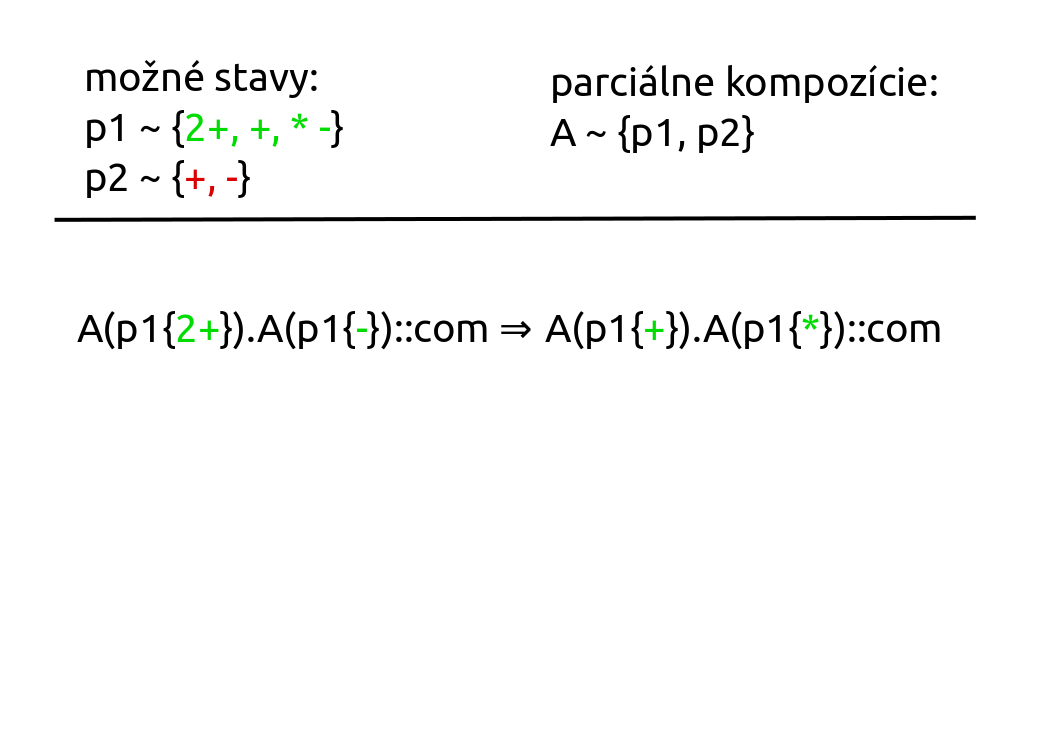
\includegraphics[width=0.75\textwidth]{equation_1}
}

\alt<2>{
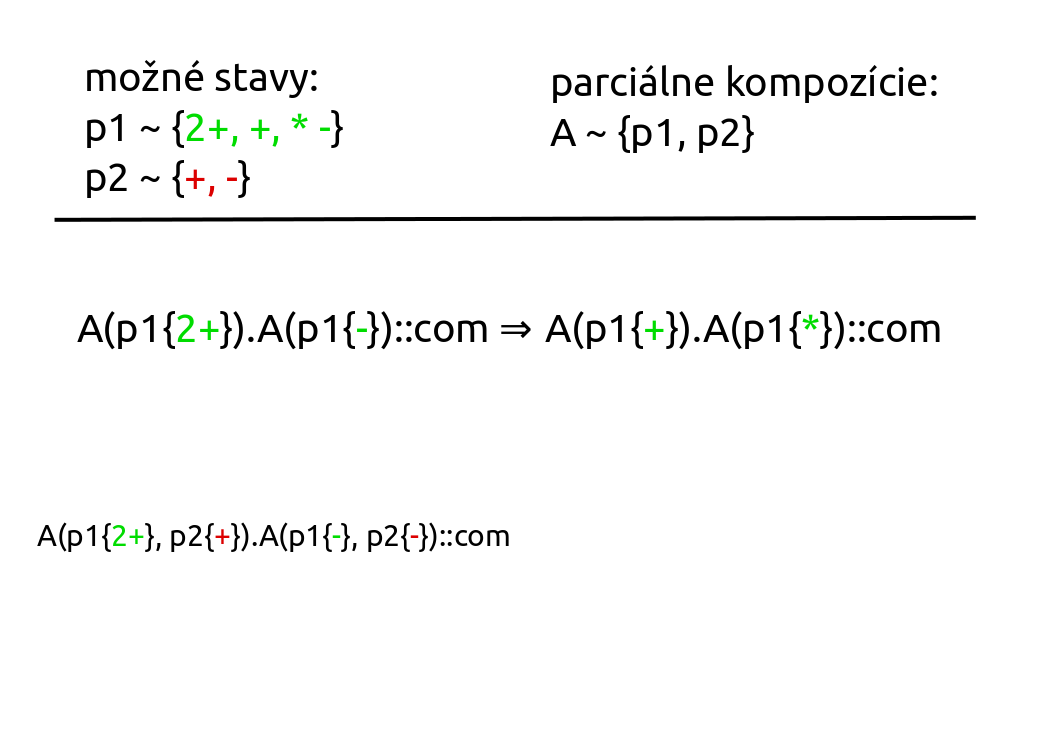
\includegraphics[width=0.75\textwidth]{equation_2}
}

\alt<3>{
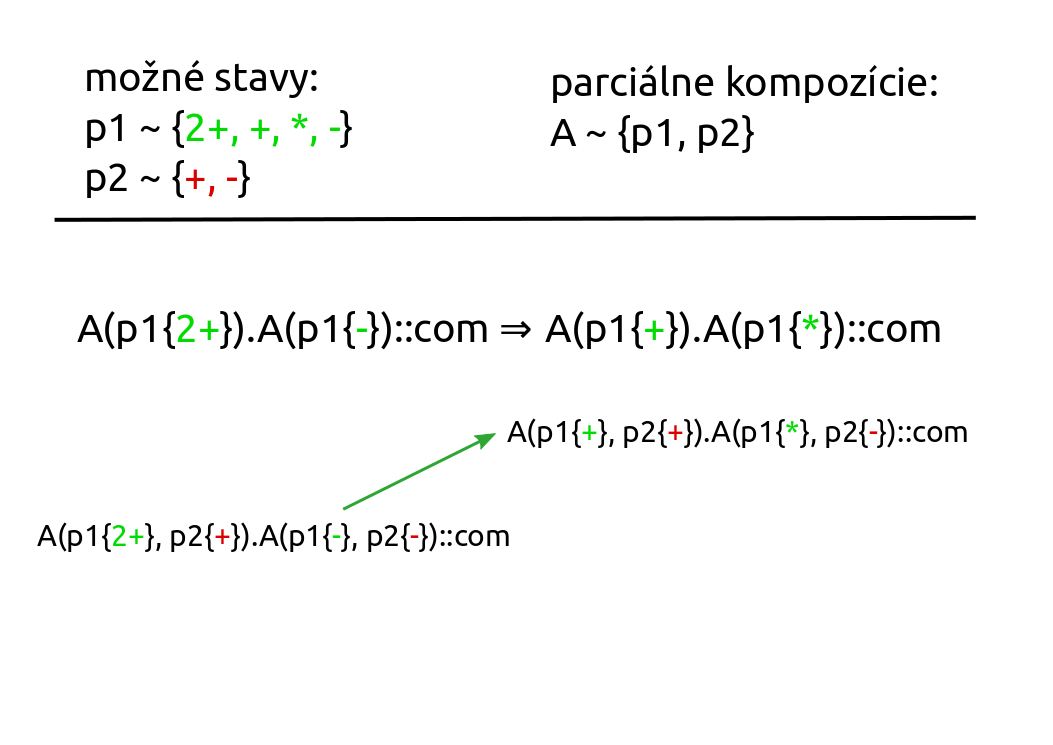
\includegraphics[width=0.75\textwidth]{equation_3}
}

\alt<4>{
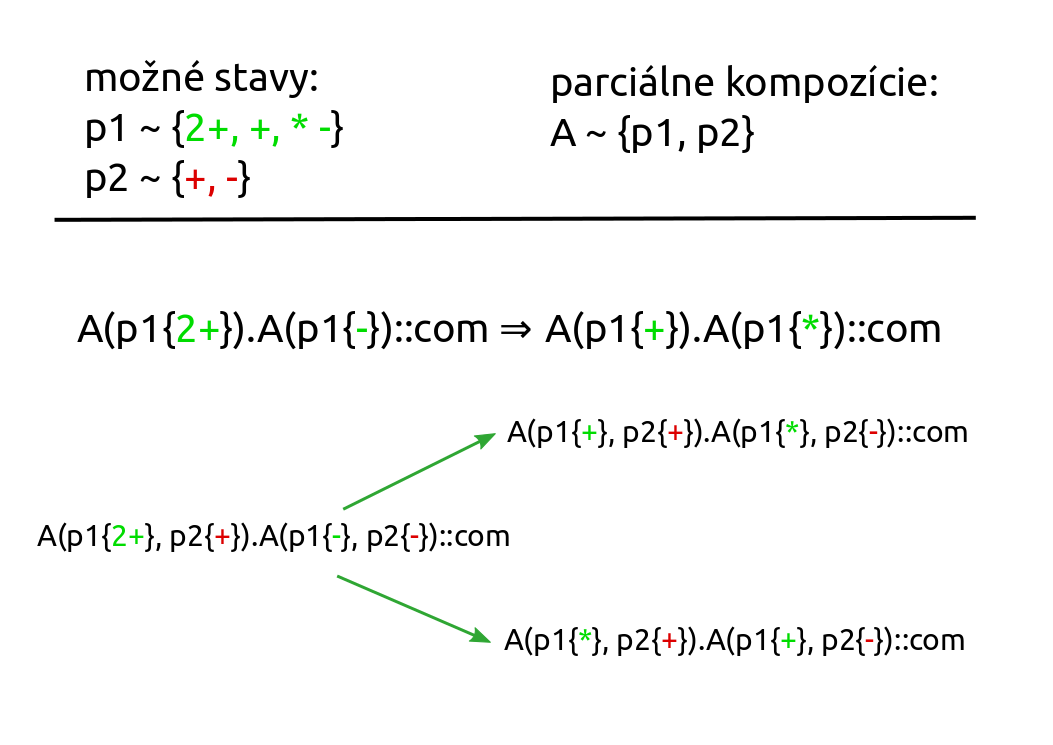
\includegraphics[width=0.75\textwidth]{equation_final}
}

\end{center}

}

% -------------------------------------------------------------

\frame{
\frametitle{Otázky oponenta}

\begin{itemize}

\item Nebolo by jednoduššie využiť v definícií grounding function kompatibilitu agentov (a zvlášť kompatibilnú podmnožinu agenta) tak ako je definovaná v nasledujúcej kapitole?

\end{itemize}

\alt<1>{
\begin{center}
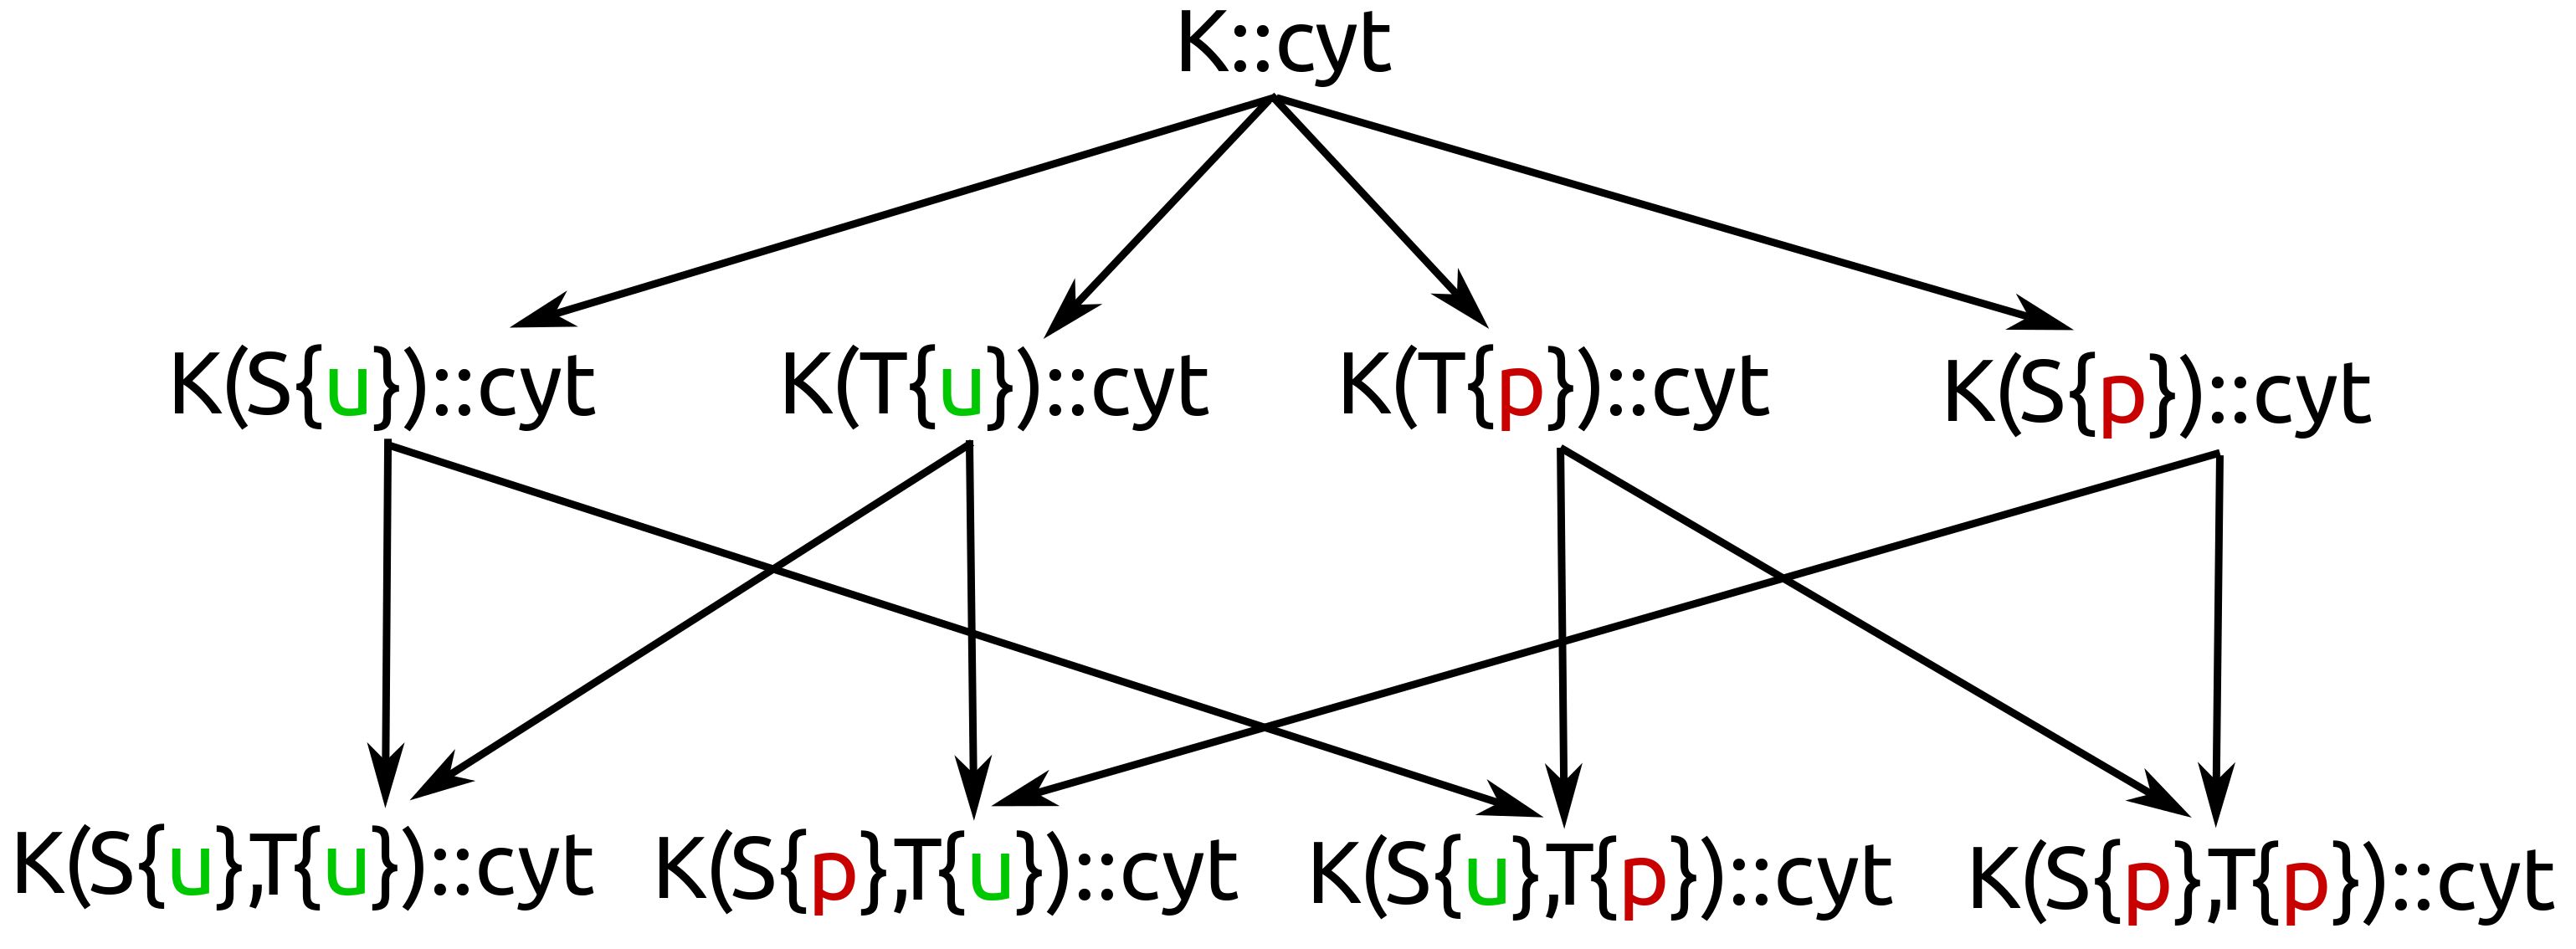
\includegraphics[width=0.75\textwidth]{partial_order}
\end{center}
}

\alt<2>{
\vspace*{0.5cm}

Áno, ale \ldots	

\vspace*{0.5cm}

\ldots nespĺňa to kritéria \emph{praktickej} definície -- bez danej definície grounding function by nebolo ukázané, ako kompatibilnú podmnožinu agenta zostrojiť.
}

}

% -------------------------------------------------------------

\begin{frame}[standout]
\thispagestyle{empty}
\begin{center}
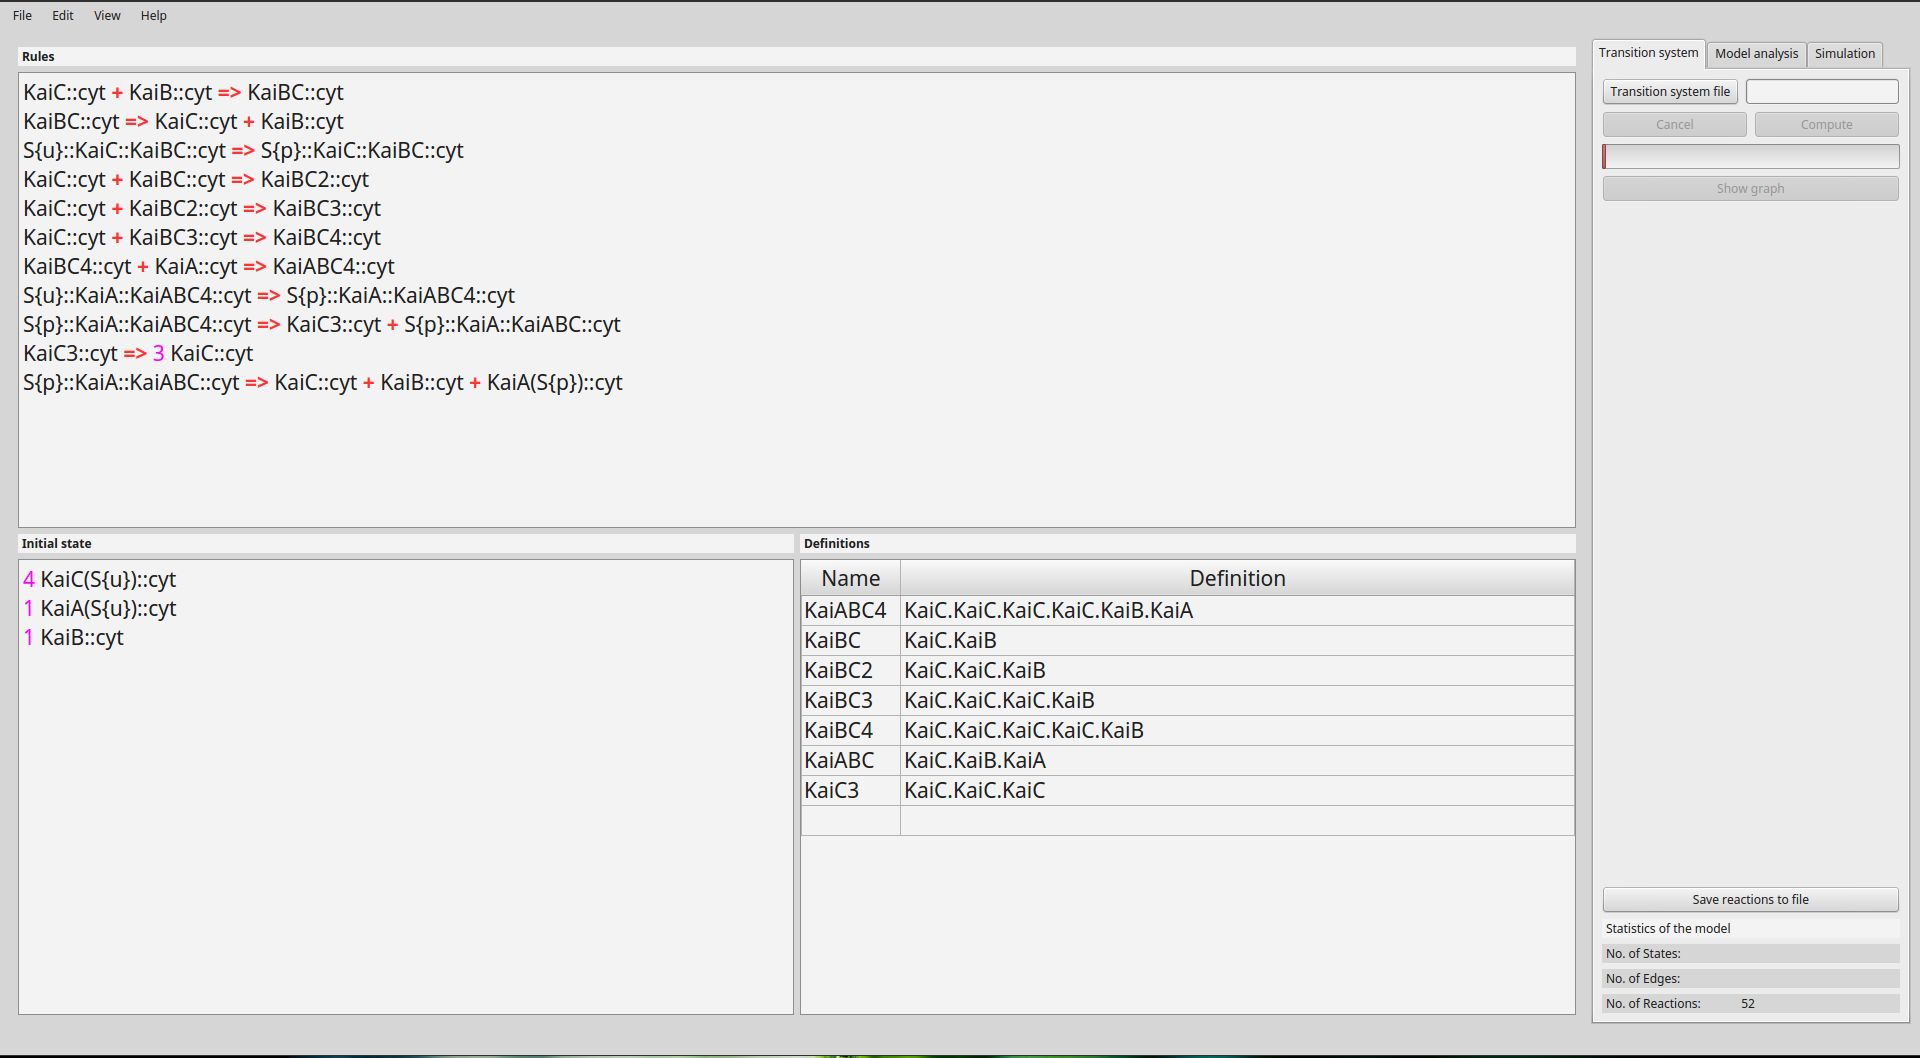
\includegraphics[width=1\textwidth]{BCSgen_intro}
\end{center}
\end{frame}

% -------------------------------------------------------------

\begin{frame}[standout]
\thispagestyle{empty}
\begin{center}
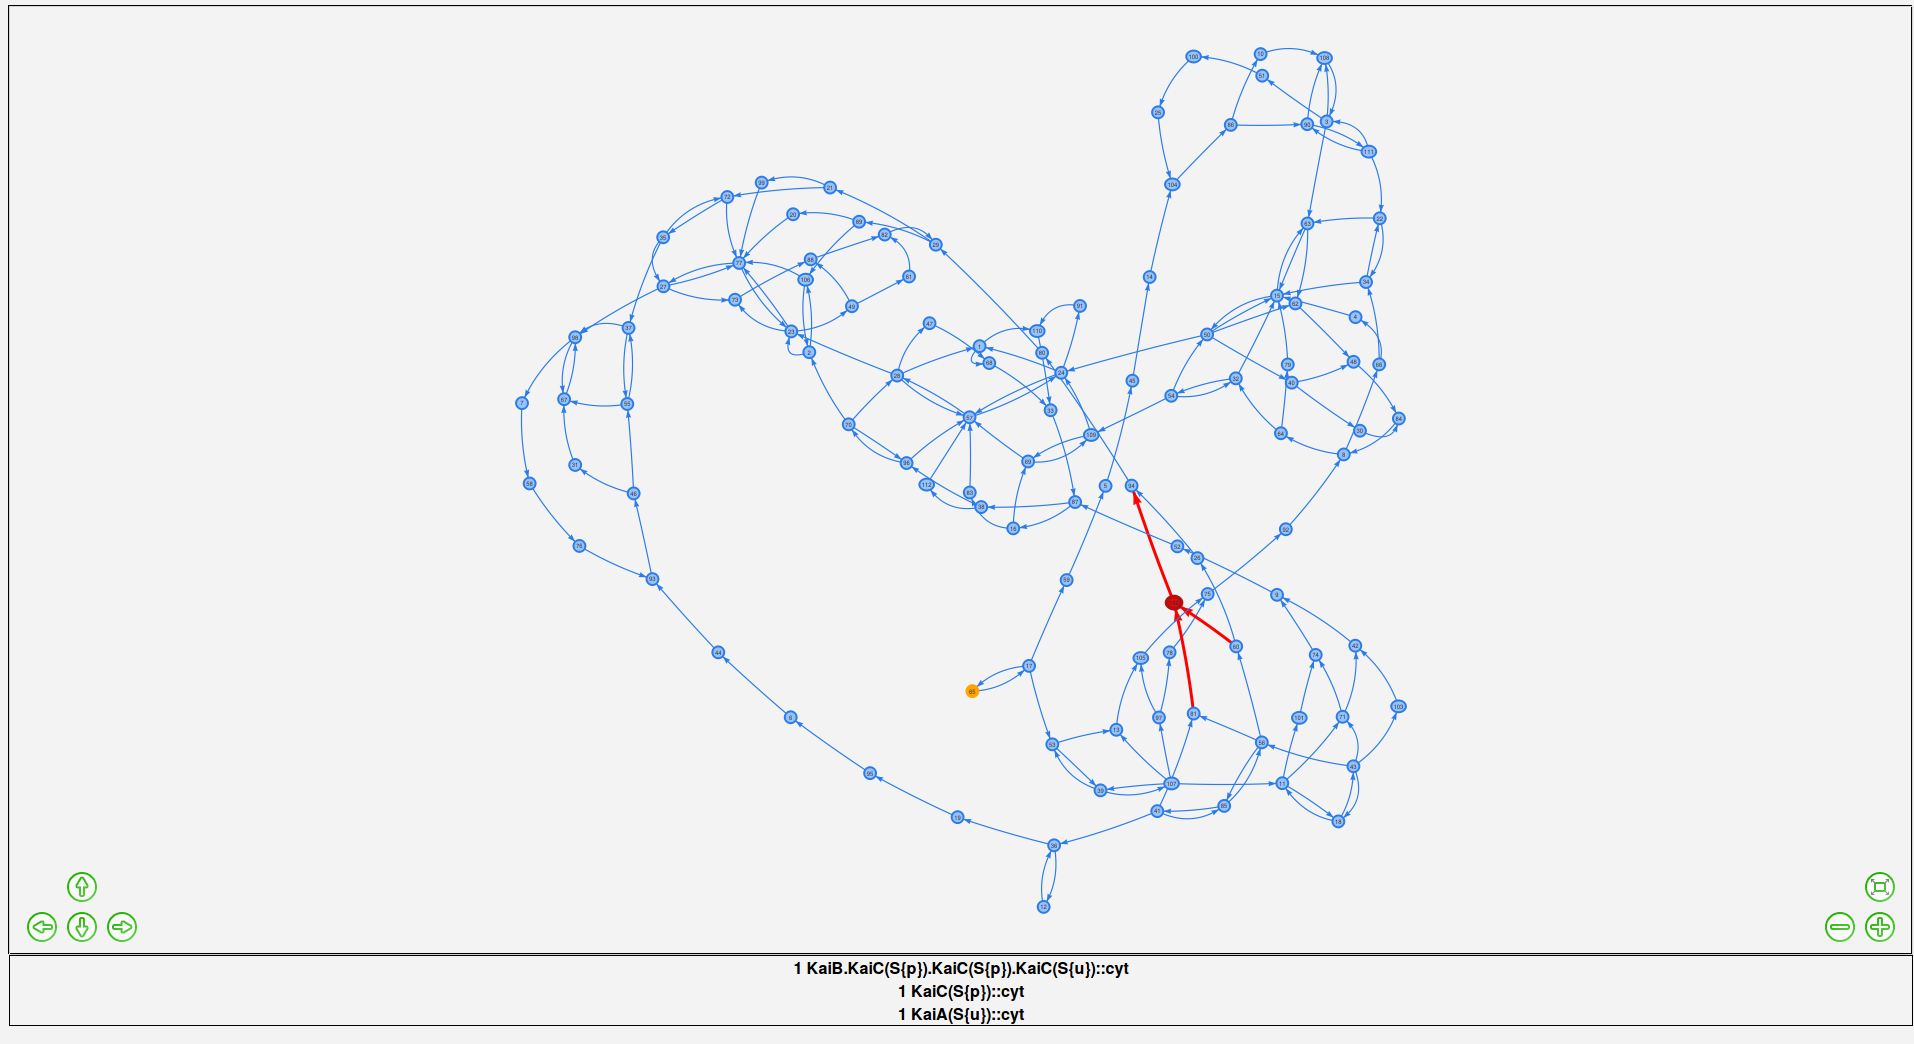
\includegraphics[width=1\textwidth]{BCSgen_ss}
\end{center}
\end{frame}

% -------------------------------------------------------------

\begin{frame}[standout]
\thispagestyle{empty}
\begin{center}
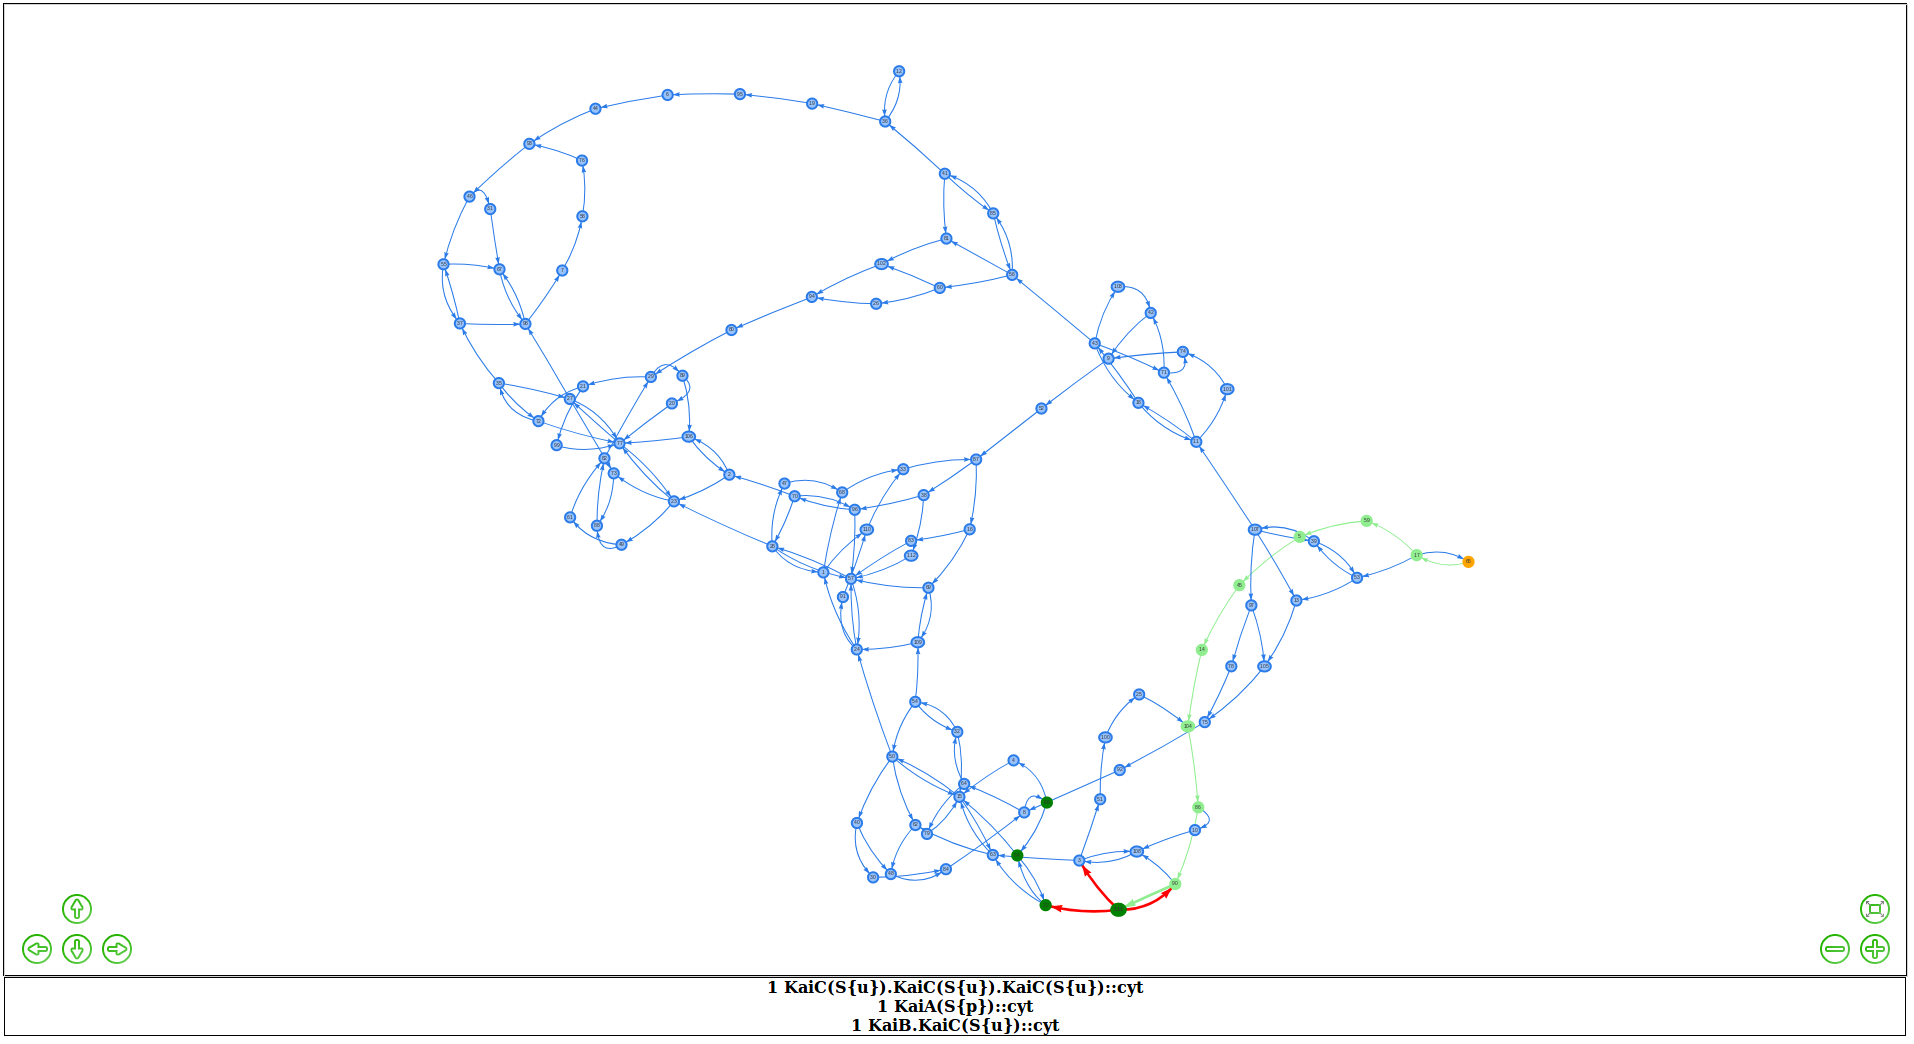
\includegraphics[width=1\textwidth]{BCSgen_reach}
\end{center}
\end{frame}

% -------------------------------------------------------------

\begin{frame}[standout]
\thispagestyle{empty}
\begin{center}
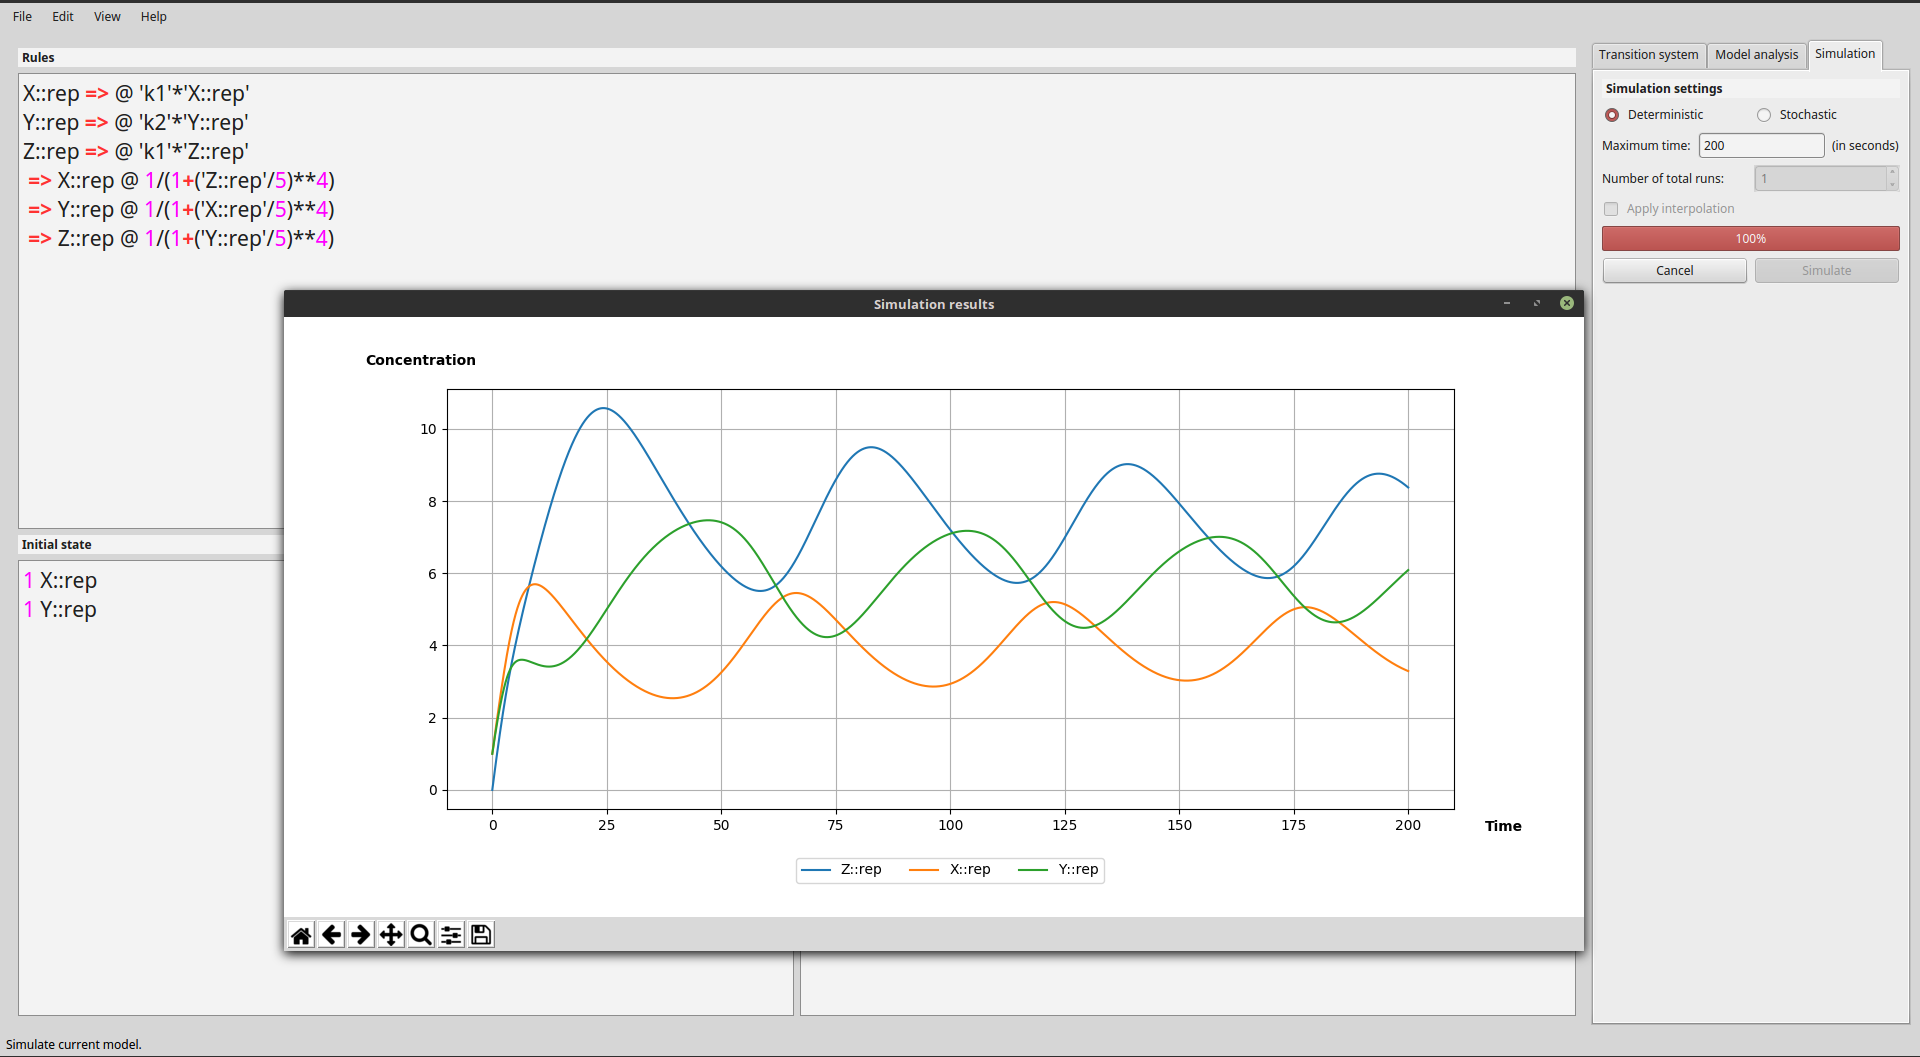
\includegraphics[width=1\textwidth]{BCSgen_deter}
\end{center}
\end{frame}

% -------------------------------------------------------------

\begin{frame}[standout]
\thispagestyle{empty}
\begin{center}
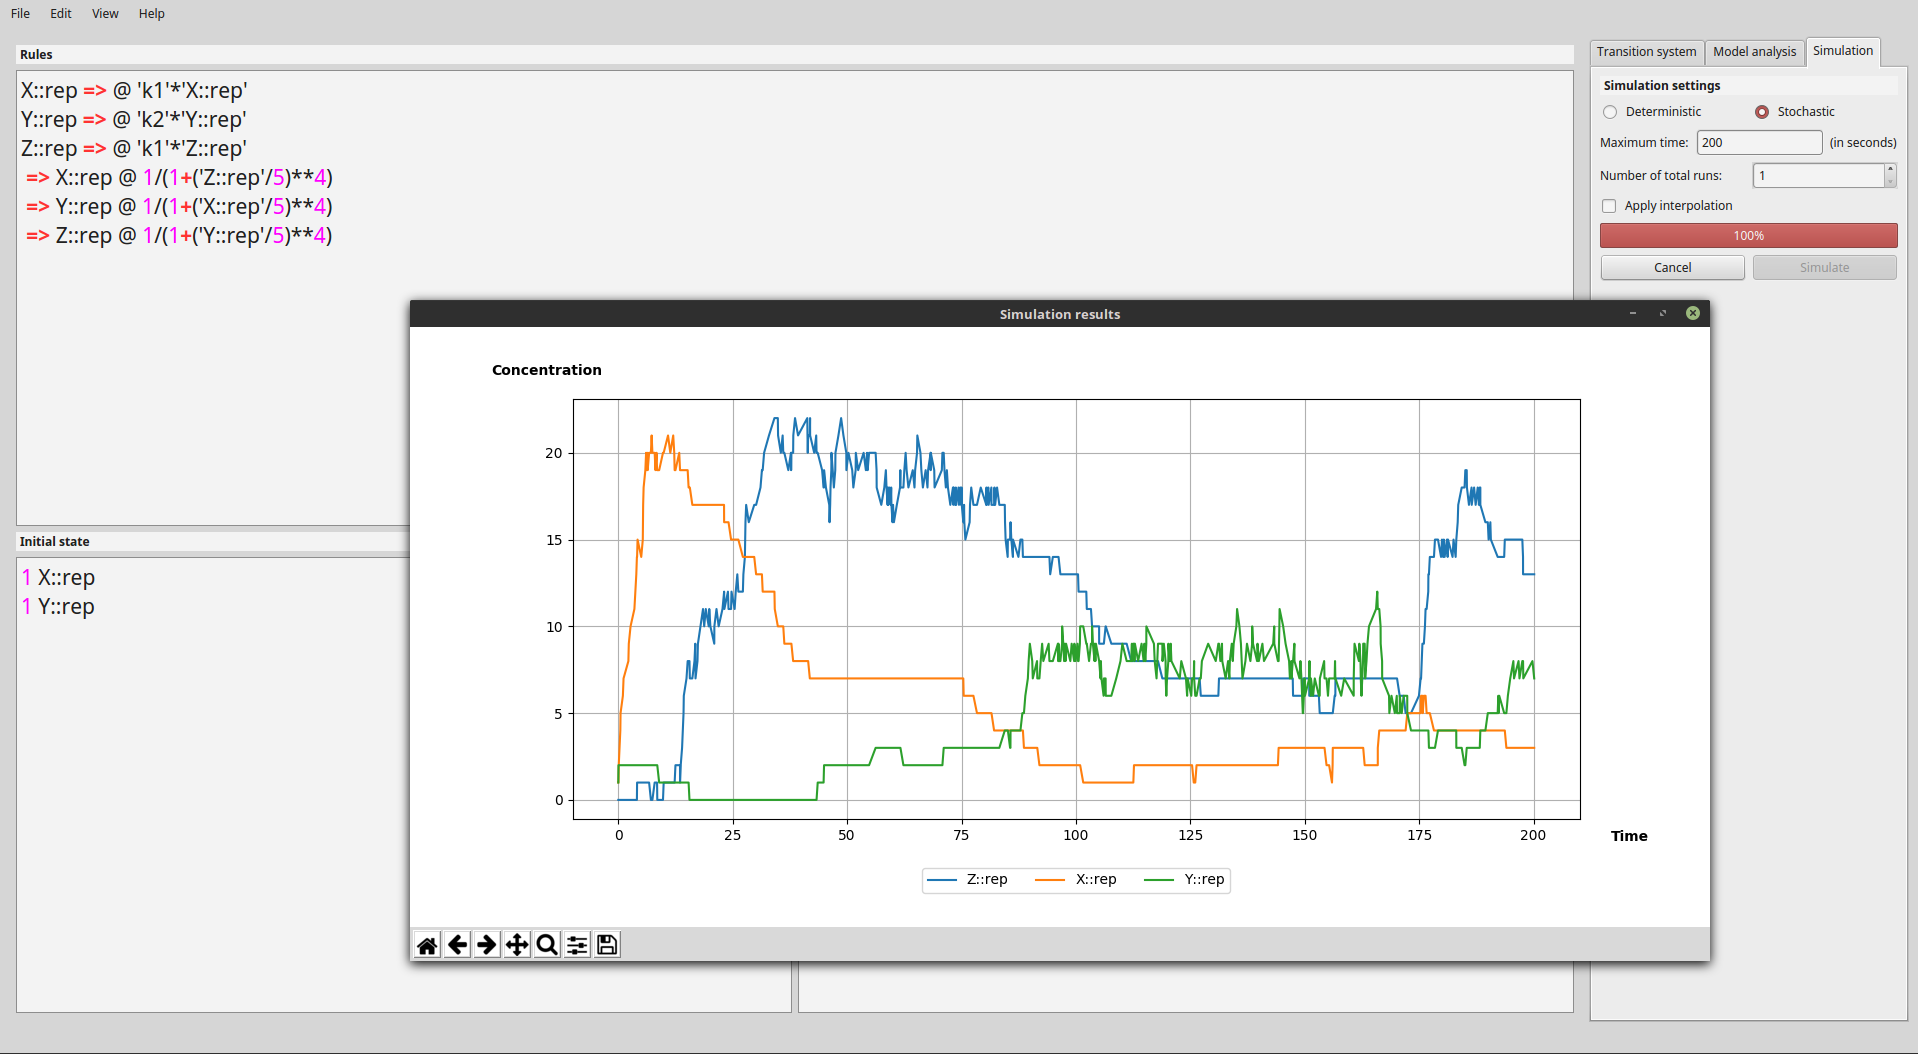
\includegraphics[width=1\textwidth]{BCSgen_stoch}
\end{center}
\end{frame}

\end{document}